\documentclass[10pt,twocolumn]{article}

% use the oxycomps style file
\usepackage{oxycomps}

% usage: \fixme[comments describing issue]{text to be fixed}
% define \fixme as not doing anything special
\newcommand{\fixme}[2][]{#2}
% overwrite it so it shows up as red
\renewcommand{\fixme}[2][]{\textcolor{red}{#2}}
% overwrite it again so related text shows as footnotes
%\renewcommand{\fixme}[2][]{\textcolor{red}{#2\footnote{#1}}}

% read references.bib for the bibtex data
\bibliography{references}

% include metadata in the generated pdf file
\pdfinfo{
    /Title (Git and LaTeX Worksheet)
    /Author (Justin Li)
}

% set the title and author information
\title{Git and \LaTeX Worksheet}
\author{Justin Li}
\affiliation{Occidental College}
\email{justinnhli@oxy.edu}

\begin{document}

\maketitle

\section{Instructions}

This worksheet is due March 1, 2025 at midnight, to be submitted as a GitHub repository URL to Canvas. The repository should contain all files requires to compile this worksheet with your answers. You should only change this \texttt{document.tex} file and the  \texttt{references.bib} file; do not change any other file in this starting repository. You should not use any additional packages, and are not allowed to use the \texttt{{\textbackslash}usepackage\{\}} command. Additionally, the output should be formatted correctly: your answers should be appropriately nested under the questions, command-line commands should be in monospace, and images should be positioned appropriately.

\section{Git Questions}

\subsection{General questions}

\begin{enumerate}
    \item What is a version control system? Why are they useful?\\
    
    A version control system is a tool used by developers that tracks changes made to files over time. A VCS is useful because it enables smoother collaboration within a team, is consistent across different versions, and keeps a clear history of edits.\\
    
    \item What is the difference between git and GitHub?\\

    Git is a version control system used through the terminal while GitHub is a platform that is designed around git and is hosted online\\
    
    \item What is a repository?\\

    A repository is a space that contains all the files of a project\\
    
    \item What is a commit?\\

    A commit is a change you made to the repository \\
    
    \item What is the commit graph?\\

    A commit graph is a representation of all the commits made to a repository\\
    
    \item What is your preferred local git client (eg., command line, GitHub Desktop, GitKraken, etc.)?\\

    I just use the command line in VS Code\\
\end{enumerate}

\subsection{Local Usage}

\begin{enumerate}
\item What is the difference between adding a file to the staging area and committing a file?\\
Adding a file to the staging area is you getting ready to commit the file. It allows you to organize, sort, and label different groups of commits before committing. Committing a file permanently saves the changes to the repository.\\

\item What is a commit message, and why is it important for them to be meaningful?\\

A commit message is a message added alongside your commit. It is important for them to be meaningful because it provides context to other collaborators (and to yourself) about the changes made in the commit.\\

\item Starting with an empty repository, what sequence of commands/actions would result in the following \\
commit graph? You may give a sequence of \texttt{git} commands or describe (with screenshots) how you would do this in your preferred graphical git interface.\\

Observe Figure 1\\
\begin{verbatim}
A---B---C---D
\end{verbatim}

\begin{figure}[htp]
    \centering
    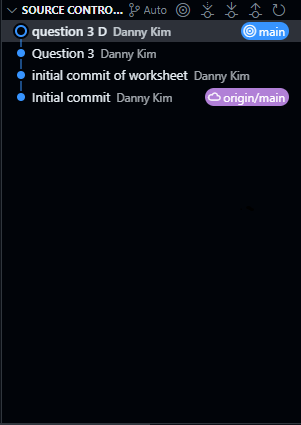
\includegraphics[width=4cm]{Q3.png}
    \caption{2.2 Question 3}
\end{figure}

\item If you are currently at commit D above, how would you recover code from commit B? What sequence of commands/actions would let you do so? You may give a sequence of \texttt{git} command-line commands, or describe (with screenshots) how you would do this in your preferred graphical git interface. Assume the commit hashes are AAAAAA..., BBBBBB..., etc.\\

Click on the desired commit, click the checkout button
Observe Figure 2\\

\begin{figure}[htp]
    \centering
    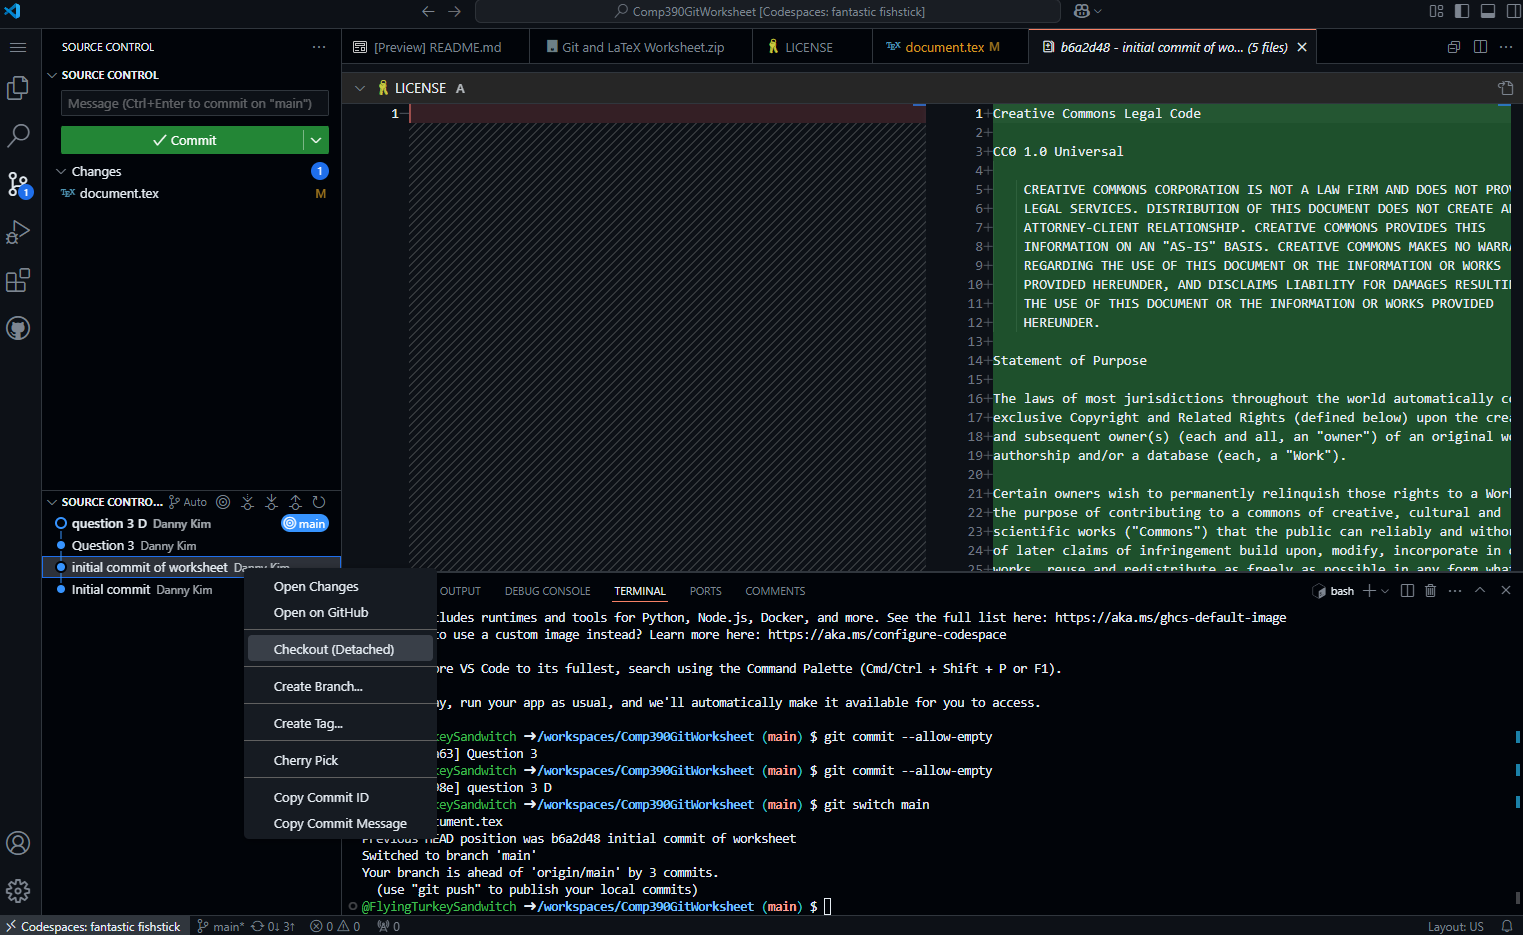
\includegraphics[width=8cm]{Q4.png}
    \caption{2.2 Question 4}
\end{figure}


\item Imagine you created a git repository for your project, but only commit your changes once a week on Sundays. You got your code working on Tuesday, but then broke your code on Friday. What can you do to get the working version of your code back?\\

You could create a new branch from the commit on Tuesday, then rebase that branch back to the Main branch while taking the code from Tuesday during the merge conflicts.

\end{enumerate}

\subsection{Branching and Merging}

\begin{enumerate}
\item What is a branch? Why are they useful?\\

A branch is a copy of the repository. It is useful because it allows the user to work on new features or bug fixes without affecting the main branch. Its also useful for working in a group setting beacuse of merging (if done correctly).\\


\item Starting with an empty repository, what sequence of commands/actions would result in the following commit graph? You may give a sequence of \texttt{git} command-line commands, or describe (with screenshots) how you would do this in your preferred graphical git interface.\\

Observe Figure 3

\begin{verbatim}
A---B---C---D
     \
      E---F
\end{verbatim}

\begin{figure}[htp]
    \centering
    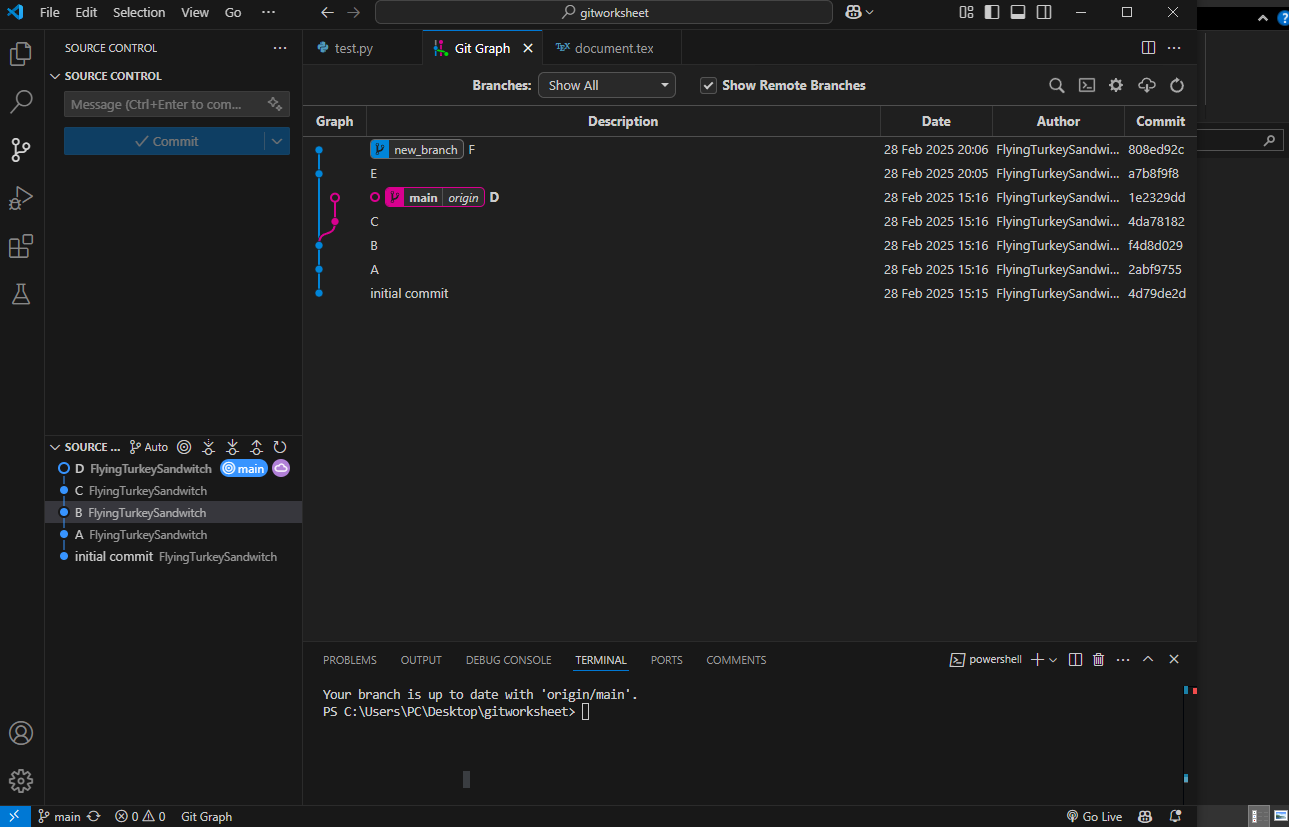
\includegraphics[width=8cm]{Q2.png}
    \caption{2.3 Question 2}
\end{figure}\textbf{}


\item Why is a merge? Why are they useful?\\

A merge is when two branches are combined into one. They are useful because they allow easy integration of contributions from different people\\

\item Imagine you are currently at commit D above. What sequence of commands/actions would result in the following commit graph? You may give a sequence of \texttt{git} commands, or describe (with screenshots) how you would do this in your preferred graphical git interface.\\

start on main branch (so D). git merge <branch name>
Observe Figure 4\\


\begin{verbatim}
A---B---C---D---G
     \         /
      E---F---/
\end{verbatim}

\begin{figure}[htp]
    \centering
    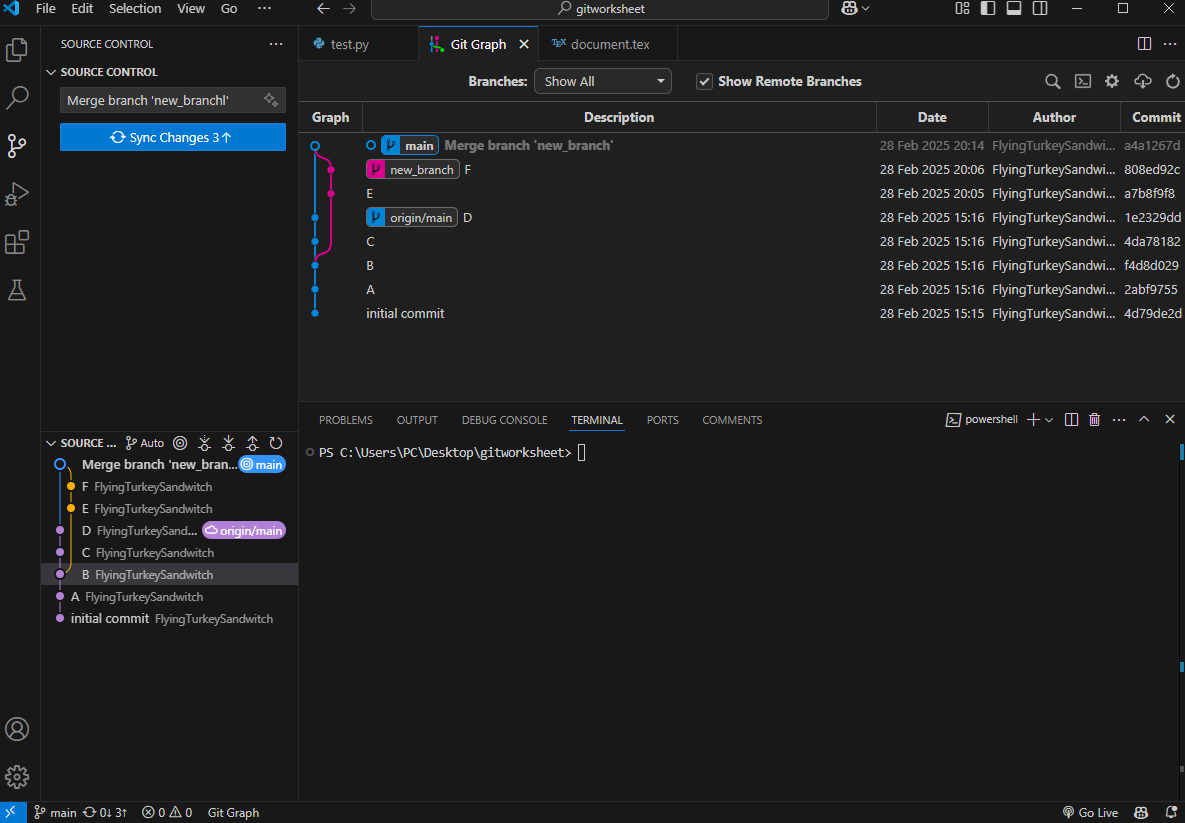
\includegraphics[width=8cm]{Q4.2.3.png}
    \caption{2.3 Question 4}
\end{figure}\textbf{}


\item What is a merge conflict? When do they occur?\\

A merge conflict occurs during a merge when the same line of code has been altered in two different ways. Because Git doesn't know which version to keep a merge conflict occurs\\

\item Starting with an empty repository, despite a sequence of commands/actions that would result in a merge conflict. Include the exact edits and \texttt{git} commands or screenshots of the graphical git interface. Include the output or screenshot that shows the resulting merge conflict.\\

1) make edits to a file
2) on a different branch, make a different edit on the same file same line
3) try to merge two branches

Observe Figures 5, 6, 7\\


\begin{figure}[htp]
    \centering
    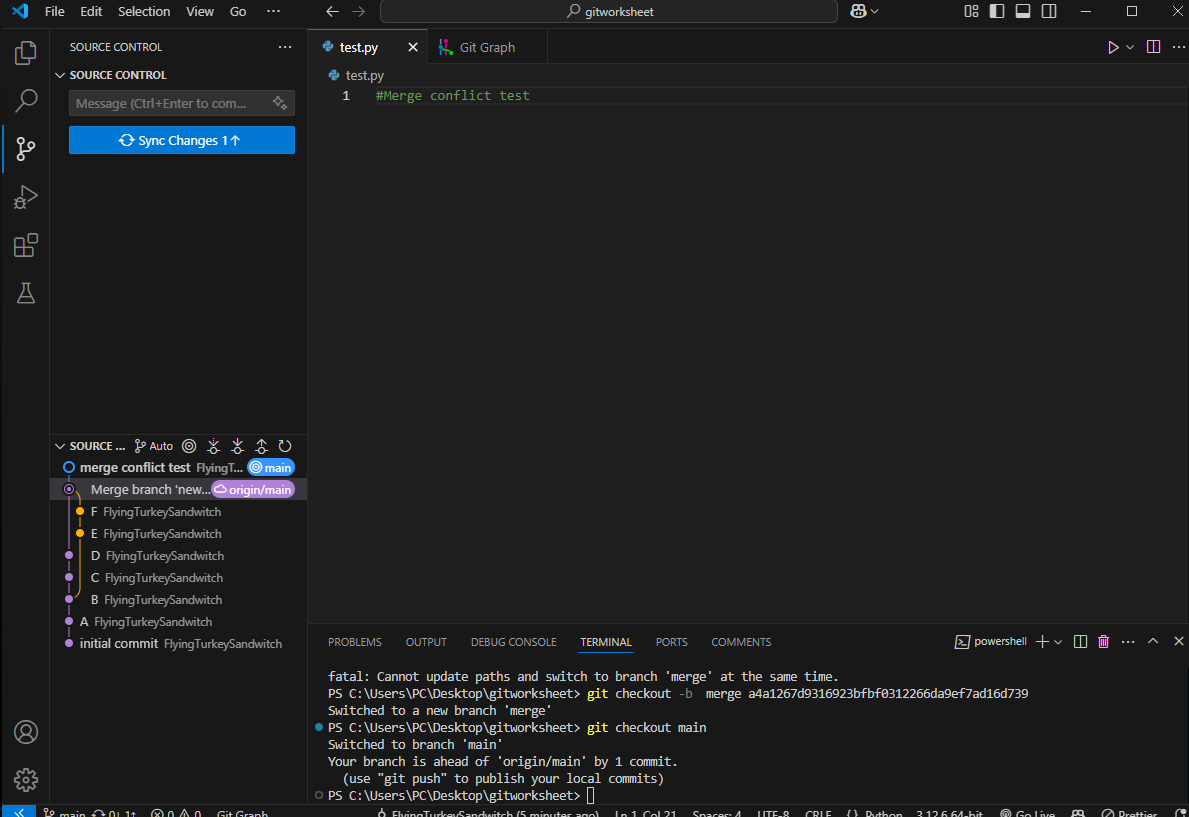
\includegraphics[width=8cm]{Q6.1.png}
    \caption{2.3 Question 6 A}
\end{figure}\textbf{}
\begin{figure}[htp]
    \centering
    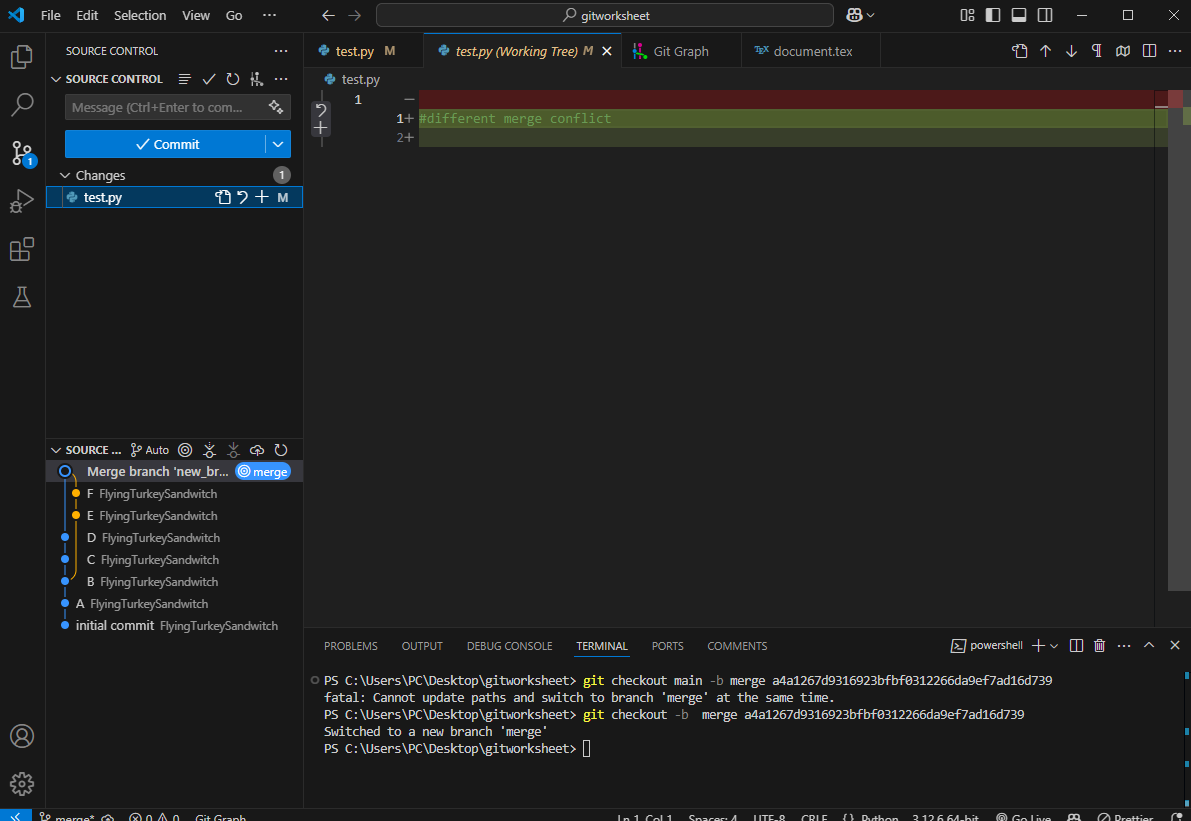
\includegraphics[width=8cm]{Q6.2.png}
    \caption{2.3 Question 6 B}
\end{figure}\textbf{}
\begin{figure}[htp]
    \centering
    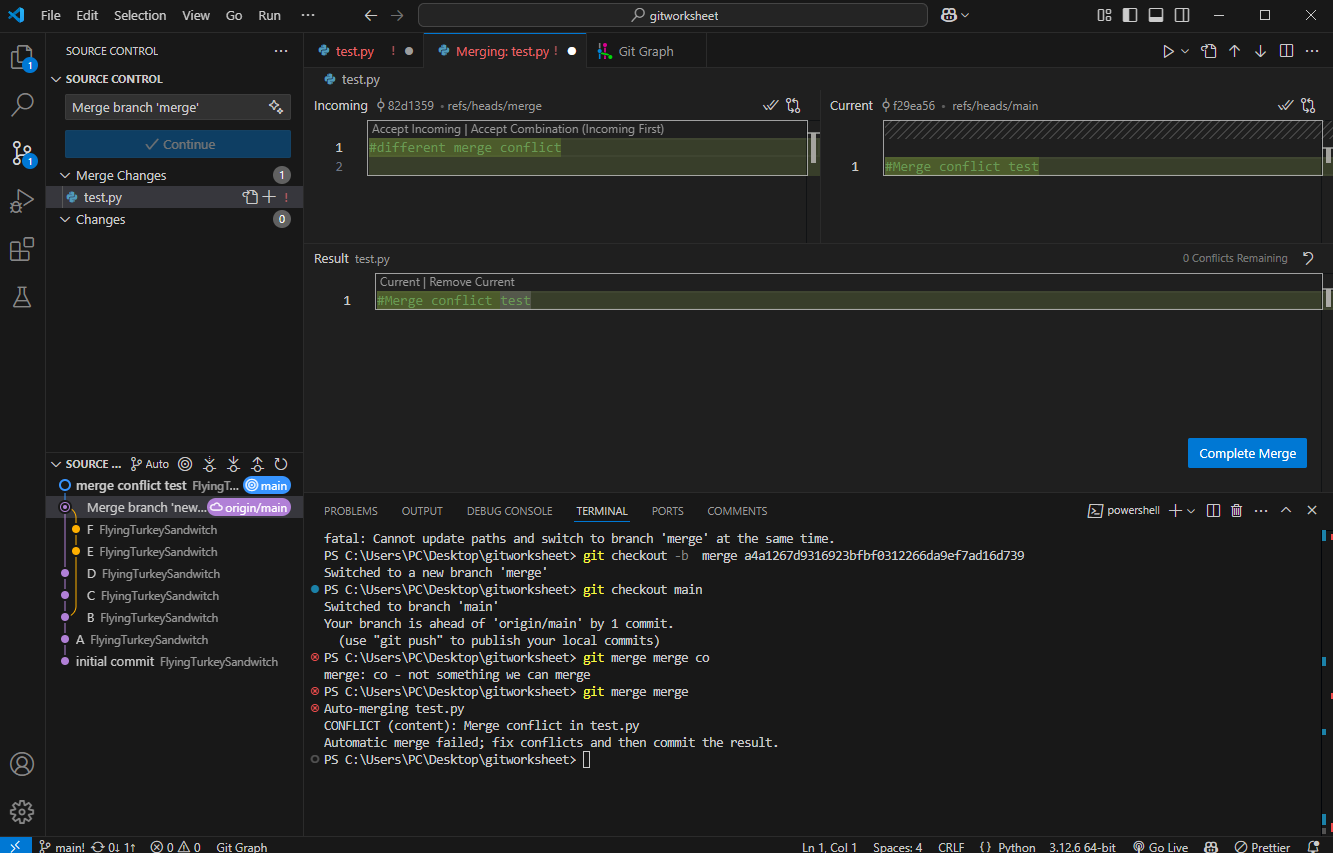
\includegraphics[width=8cm]{Q6.3.png}
    \caption{2.3 Question 6 }
\end{figure}\textbf{}



\end{enumerate}

\subsection{Remotes}

\begin{enumerate}
\item What is a remote?\\

A remote is a copy of your repository stored on an online platform (such as GitHub).\\

\item What does pushing and pulling do?\\

Pushing is updating the remote repository with your local repository while pulling is updating your local repository with the remote repository. \\

\item Imagine you created a git repository for your project on your laptop and commit regularly, but only push your code to GitHub once a week on Sundays. Your laptop caught on fire on Friday. What can you do to get your code back?\\

You can pull from the remote repository to get your code back. However, you can only recover code saved from the previous Sunday (so you lose the work you did for monday-friday).\\

\end{enumerate}

\section{\LaTeX}

Find a source of each of the following types and add it to \texttt{references.bib}, with the appropriate data. Your sources do not have to relate to your project. Looking at \textcite{OverleafBibliographyManagement} and \textcite{WikipediaBibtex} may be helpful,

\begin{itemize}
\item a journal article
\cite{Aryal2024}
\item a conference article
\cite{Shahpas2019}
\item a PhD or Master's thesis
\cite{Zhong2021}
\item an article in an edited popular media venue (newspaper, magazine, etc.)
\cite{Sciforce2022}
\item a book
\cite{Sotiropoulos2024}
\item a chapter of a book
\cite{SotiropoulosCH2024}
\item a YouTube video
\cite{Orchard2021}
\item a piece of technical documentation (e.g., a programming language reference, and API documentation, etc.)
\cite{TextAttack2021}
\end{itemize}

Additionally, in you own words, explain the difference between \texttt{{\textbackslash}cite\{\}} and \texttt{{\textbackslash}textcite\{\}}. When should they each be used? Demonstrate your answers by using one of them with each of your references from above.\\

\texttt{{\textbackslash}cite\{\}} should be used when citing something in text. \\

ex: Overleaf is the preferred program of Computer Scientists \cite{OverleafBibliographyManagement}\\

\texttt{{\textbackslash}textcite\{\}} should be used when the author's name is integrated into the sentence. \\

ex: \textcite{WikipediaBibtex} provides a wide description of BibTeX


\printbibliography


\end{document}
